%%%%%%%%%%%%%%%%%%%%%%%%%%%%%%%%%%%%%%%%%%%%%%%%%%%%%%%%%%%%%%%%%%%%%%%%%%%%%%
%
% Section file included in main project file using \input{}
%
% Assumes that LaTeX2e macros and packages defined in cg_comp.sty are
%   available
%
%%%%%%%%%%%%%%%%%%%%%%%%%%%%%%%%%%%%%%%%%%%%%%%%%%%%%%%%%%%%%%%%%%%%%%%%%%%%%%

 \section{Introduction and Background\label{sct:intro}}

Any musician who has wrestled with the temperament of a fretted stringed instrument is well aware of the challenges presented by tuning and pitch. In addition to the mathematical physics of musical scales~\cite{ref:krantz1994mre,ref:hall2001mmi,ref:durfee2015pms}, the mechanical specifications of the instrument and the strings themselves~\cite{ref:morse1981vas,ref:fletcher2005pmi,ref:ramsey2023fag} require accommodation during both manufacturing~\cite{ref:byersgal,ref:byers1996cgi,ref:varieschi2010icf} and tuning to achieve harmonious results. We can gain an appreciation for this problem by analyzing the expression for the allowed vibration frequencies of an ideal string, given by~\cite{ref:morse1981vsa,ref:fletcher2005pma}
 \begin{equation} \label{eqn:f_0_def}
f_q = \frac{q}{2\, L_0}\, \sqrt{\frac{T_0}{\mu_0}}\, ,
 \end{equation}
where $q \in \mathbb{N} = \{1, 2, \dots\}$ identifies the ``harmonic'' of the fundamental frequency $f_1$, $L_0$ is the length of the free (unfretted) string from the saddle to the nut, $T_0$ is the tension in the free string, and $\mu_0 \equiv M / L_0$ is the linear mass density of a free string of mass $M$. The act of fretting the string changes its length, and therefore its frequency. For example, modern classical guitars are manufactured with frets placed along the fretboard using the Twelve-Tone Equal Temperament (12-TET) system, whereby the resonant length of a string pressed behind fret $n$ ideally should be $2^{-n/12}\, L_0$, thereby producing a note with frequency $2^{n/12}\, f_1$. But this result can never be achieved perfectly in reality. 

First, the string is elevated above the frets by the saddle and nut, so the fretted string is slightly elongated relative to the free string, and the resulting frequency is flattened in pitch. In principle, this effect could be accommodated by minute changes in the positions of the frets, but there are additional practical complications. For example, the string's tension is increased by the change in length, causing the frequency to sharpen by an amount that significantly exceeds the reduction caused by the increase in the resonant string length. In addition, the string is by no means ideal, and its intrinsic stiffness results in an additional increase in pitch that depends on its mechanical characteristics. These guitar intonation difficulties seem to preclude successful temperament, but remarkably the instrument can be \emph{compensated} by moving the positions of the saddle and the nut by small distances during the manufacturing process~\cite{ref:byersgal,ref:byers1996cgi,ref:varieschi2010icf}. This compensation process helps temper the guitar so that it is \emph{playable}. It must also be \emph{tunable}, so that the guitar strings can be brought into compliance with 12-TET quickly and accurately. This requirement places significant constraints on the physical properties of manufactured strings. Our goal in this work is to build an intuitive understanding of these effects to aid in the compensation and subsequent tuning of the classical guitar, with an accessible approach to making measurements of string properties and deducing the corresponding effects of playability~\cite{ref:erkut2000epe,ref:noll2014gim,ref:dostal2020srw}.

Throughout this work, we will use \emph{cents} to describe small differences in pitch~\cite{ref:durfee2015pms,ref:varieschi2010icf,ref:hall1985see,ref:hall1988anl,ref:krantz2000cie,ref:jedrzejewski2008gds}. One cent is one one-hundredth of a 12-TET half-step, so that there are 1200~cents per octave.  The difference in pitch between two frequencies $f_1$ and $f_2$ is logarithmic, and is defined as
 \begin{equation} \label{eqn:cents_def}
\Delta \nu \equiv 1200\, \log_2\left(\frac{f_2}{f_1}\right)\, ,
 \end{equation}
 where $\log_2(x)$ is the (binary) logarithm base 2 of $x$. Let's choose the average frequency $f \equiv (f_1 + f_2) / 2$ and the frequency difference $\Delta f \equiv f_2 - f_1$. Then
 \begin{equation} \label{eqn:cents_approx}
\Delta \nu = 1200\, \log_2\left(\frac{f + \Delta f / 2}{f - \Delta f /2}\right) \approx \frac{1200}{\ln(2)}\, \frac{\Delta f}{f} \approx 1731\, \frac{\Delta f}{f}\, ,
 \end{equation}
where the approximation applies when $\Delta f \ll f$, and $\ln(x)$ is the natural logarithm function of $x$.  An experienced classical guitar player can distinguish beat notes with a difference frequency of $\Delta f \lesssim 1$~Hz, which corresponds to 8~cents at $A_3$ ($f = 220$~Hz) or 5~cents at $E_4$ ($f = 329.63$~Hz). As shown in \fig{diff_pitch}, if the average frequency of the interval is used to compute $\Delta \nu$ --- rather than the initial frequency $f_1$ --- then the accuracy of \eqn{cents_approx} holds for almost an entire octave. In this plot, we chose $f_1 = A_3 = 220$~Hz, and allowed $f_2$ to vary from $A_3$ to $A_4 + 30 \textrm{ Hz} = 470$~Hz. At the octave, the error in $\Delta \nu$ arising from \eqn{cents_approx} is only $-46$~cents, or $-4$\%. The choice of a logarithmic frequency-difference scale \emph{decouples} multiplicative factors that predict the frequency of a real fretted string, allowing us to build straightforward intuitive models of guitar intonation and compensation.

We present the basics of our model of classical guitar strings in \sct{model}, following the pioneering work of G.\ Byers~\cite{ref:byersgal,ref:byers1996cgi,ref:byersweb}. We offer empirical reasons to doubt the need for a complicated model of string fretting that incorporates either the depth of fretting or the shape of the finger in \app{fret}. Then, in \app{freq}, we derive a new expression for the allowed vibration frequencies of a stiff string (although more complicated dynamical models are available~\cite{ref:ducceschi2016lss}), derived  under the assumption that the boundary conditions at the saddle and the nut are not symmetric. Based on this result, we then discuss in detail the four contributions to frequency shifts and errors of strings pressed behind a fret: the change in the resonant length of the vibrating string; a decrease in the linear mass density of the entire string; an increase in the tension of the entire string; and an increase in the mechanical stiffness of the resonating string. Our goal is to simplify the decoupled equations describing these effects through Taylor series expansions to allow an intuitive picture of the string's behavior to emerge. Nylon strings~\cite{ref:blanc1996nvb,ref:lynchaird2017mpn,ref:lynchaird2018cmp} behave very differently than the metal strings used on acoustic and electric guitars~\cite{ref:grimes2014stp,ref:kemp2017puw,ref:kemp2020ibg}. After restringing, they first stretch and deform inelastically and then require hours to ``settle'' and reach a linear elastic equilibrium, and it is unlikely that the uniform stiff rod approach used to develop equations for the resonant frequencies (including ours) apply to either the monofilament treble strings or the wound bass strings until that equilibrium is reached. Nevertheless, we are able to develop a phenomenological model of the mechanical characteristics of these strings that is consistent with measurements of frequency deviations on uncompensated classical guitars.

In our analysis, we neglect two contributions to the sound produced by classical guitars. First, we do not account for the impact of the plucked string polarization on the boundary conditions we used to describe the vibrations of a string. A standard free stroke on a nylon classical guitar string results in an elliptically polarized response, with the major (horizontal) axis in the plane of the strings parallel to the fret board. In principle, the vertical and horizontal oscillations could vibrate at different frequencies, but we see no evidence of peak splitting in spectrum analysis of the first half dozen harmonics of fretted normal tension strings on the several classical guitars we tested. Second, given this result, we neglected all details of guitar body manufacturing such as bridge admittance~\cite{ref:woodland2004pgt,ref:torres2009ibv} because they are unlikely to affect computations of setbacks in guitar compensation.

\begin{figure}
    \centering
    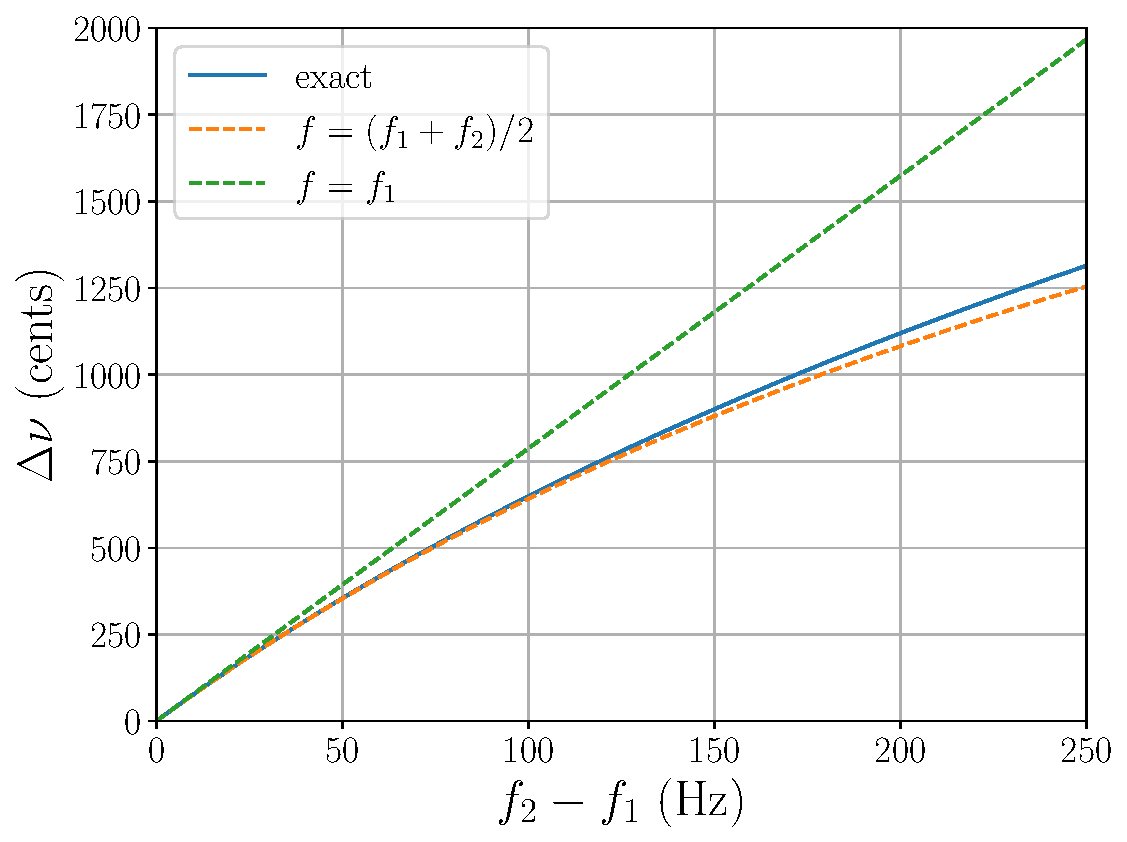
\includegraphics[width=6.5in]{figures/diff_pitch}
    \caption{\label{fig:diff_pitch} Plot of $\Delta \nu$ for $f_1 = A_3 = 220$~Hz and $f_2$ varying from $A_3$ to $A_4 + 30 \textrm{ Hz} = 450$~Hz. We compare two different definitions of $f$ in \eqn{cents_approx}: the average of $f_1$ and $f_2$, and simply $f = f_1$. Using the average frequency leads to a significantly better approximation.}
\end{figure}

In \sct{tot_freq_shift}, we collect all four of the effects mentioned above and develop a simple approximate expression for the total frequency shift of a fretted guitar string. We note that the two largest contributions to this deviation from 12-TET perfection are the increases in tension and bending stiffness due to fretting, and that small changes in the positions of the nut and the saddle can largely compensate for these problems. In \sct{exp}, we demonstrate a simple, straightforward experiment to measure \emph{in situ} the response of a string's fundamental frequency to a change in length (and therefore tension), and we test and rely on a subsequent phenomenological approach to determining the open-string bending stiffness. Then, in \sct{comp}, we use these values for a normal-tension nylon string set (as well as other string sets in \app{specs}) to demonstrate a straightforward analytic approach to compensating for the tone errors in a guitar string. We check this method numerically by relying on a technique --- described in \app{rms} --- to minimize the root-mean-squared (RMS) frequency deviation at each fret. With these results in hand, in \sct{temp} we discuss a collaboration of guitar manufacturer and musician to temper the guitar using harmonic tuning to optimize it for a particular piece. Finally, in \sct{conc}, we summarize our results and suggest topics for future work.

This document --- as well as the Python computer code needed to reproduce the figures --- is available at GitHub~\cite{ref:github2024rgb}. 